\documentclass[a4paper,UKenglish,cleveref, autoref, thm-restate]{lipics-v2021}
\usepackage{xspace}
\usepackage{graphicx} % For \includegraphics
%\graphicspath{{./graphics/}}%helpful if your graphic files are in another directory
\usepackage{amsmath}
\bibliographystyle{plainurl}% the bibstyle
\usepackage{cleveref} % Provides \Cref
\usepackage{listings} % For code snippets


\title{Implementation and verification of encoder, decoder and generator for prefix-free codes}

\author{Samuel Chassot}{EPFL}{samuel.chassot@epfl.ch}{}{}
\author{Daniel Filipe Nunes Silva}{EPFL}{daniel.nunessilva@epfl.ch}{}{}

\authorrunning{S.~Chassot and D.~F.~Nunes~Silva}

\Copyright{Samuel Chassot and Daniel Filipe Nunes Silva}

\ccsdesc[500]{Software and its engineering~Software verification and validation}

\keywords{formal verification, prefix-free codes, Huffman Coding}

\category{}
\relatedversion{}
\supplement{}
\nolinenumbers 
\hideLIPIcs

\begin{document}

\maketitle

\begin{abstract}
    We propose an implementation in the Scala programming language of an encoder, a decoder as well as a naive prefix-free code generator. These implementations are formally proven for correctness thanks to the verification framework Stainless \cite{stainless}. Those three functions can be chained to form a pipeline as a whole on a given input string $s$, i.e. generate a correspoding prefix-free code $c$, use $c$ to encode $s$ as $e$ and finally decode $e$ with $c$ as $d$. Correctness is therefore defined as $s == d$.
\end{abstract}

\definecolor{bgcolor}{RGB}{240,252,210}
\definecolor{kwcolor}{RGB}{0,0,200}
\lstdefinelanguage{scala}{
  keywordstyle=\color{kwcolor},
  backgroundcolor=\color{bgcolor},
  alsoletter={@,=,>},
  morekeywords={abstract, case, class, def,
        else, extends, false, free, if, implicit, match,
        object, true, val, var, while, sealed,
        for, dependent, null, type, with, try, catch, finally,
        import, final, return, new, override, this, trait,
        private, public, protected, package, throw},
  sensitive=true,
  morecomment=[l]{//},
  morecomment=[s]{/*}{*/},
  morestring=[b]",
  mathescape=true,
  %emph={Int,Char,Boolean,String,Unit},
  %emphstyle={\color{blue}}
}
\lstset{language=scala}


\section{Introduction}
\label{sec:intro}

The aim of this project is to come up with a verified implementation of an encoder and decoder pair as well as a prefix-free code generator in the scope of a personal project for the Formal Verification course (CS-550) at EPFL.

In \cite{blanchette}, J. C. Blanchette presents a formal proof of the optimality for the Huffman's algorithm. The latter generates a prefix-free code for a string such that the encoding of the encoded string has minimal length. As proposed in the conclusion of Blanchette's article, we explore the verification of encode/decode functions.

In this report, we start with some background knowledge related to prefix-free codes. Then, we go through the verified implementation of the pipeline we propose.

\subsection*{Prior work}

To the best of our knowledge, this is the first time an encode/decode function pair is formally verified.
However we can find many examples of similar exercises in the litterature such as a formal definition Huffman's algorithm in \cite{formal} or a formally verified implemention of compression/decompression function pair for deflate in \cite{deflate}.

\subsection*{Our approach} % the star makes the section number disappear

We first consider the whole class of prefix-free codes and not only the optimal ones generates by Huffman's algorithm.
Then, we come up with basic datatypes and implementations plain Scala code before adding  \emph{require}s and \emph{ensuring}s from Stainless in order to validate the main correctness theorem.
Finally, we also implement and verify an naive prefix-free code generator in order to complete the whole pipeline.

\subsection*{Contributions} % the star makes the section number disappear

The main contributions of this report are the following:
\begin{enumerate}
    \item a formally verified implementation of an encode function for prefix-free codes
    \item a formally verified implementation of an decode function for prefix-free codes
    \item a formally verified implementation of a prefix-free code generator
\end{enumerate}

\section{Implementation}

Our code is available in the following repository:
\begin{center}
    \url{https://github.com/samuelchassot/FormalVerification-Project}
\end{center}
and build instructions are in file \verb|README.md| in the top-level directory.

\section{Prefix-free codes}

We define a code as a map from a list of characters formed from a string, the symbols, to a list of bits, the code words. The fact that a code is prefix-free means that there is no full code word in this map that is a prefix of an other code word, i.e. $01$ is a prefix of the code word $0111$.

Those codes can be represented as full binary trees. To determine the code word of a symbols located in the leaves, it suffices to find the path from the root down to the corresponding leaf assuming that taking the left child represents the 0 bit and the right child represents the 1 bit.

{'a': 0, 'b': 10, 'c': 110, 'd': 111} is a prefix-free code and the correponding full binary tree can be seen in figure~\ref{fig:pfc}.
\begin{figure}[ht]
    \centering
    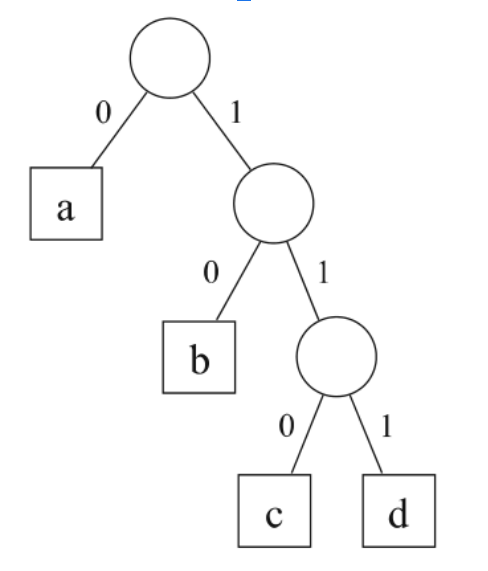
\includegraphics[width=0.3\textwidth]{pfc.png}
    \caption{A full binary tree representing a prefix-free code.\label{fig:pfc}}
\end{figure}

\section{Datatypes}

We represent a string (the tyoe of an input of the pipeline) as \lstinline{List[Char]} as it is easier to define recursion using lists rather than the \lstinline{String} type directly. 
Similarily we define an encoded binary string (the type of an output of the pipeline) as \lstinline{List[Boolean]}.

To represent the binary trees used to represent the prefix-free codes, we define the folowing case classes:

\begin{lstlisting}
    sealed abstract class Tree
    case class InnerNode(t1: Tree, t2: Tree) extends Tree
    case class Leaf(w: BigInt, c: Char) extends Tree
  
    type Forest = List[Tree]
\end{lstlisting}

A \lstinline{Forest} is a list of trees that is used in the process of generation of the prefix-free code.

We define two functions on \lstinline{Tree}s:
\begin{itemize}
    \item \lstinline{isSubTree(t: Tree, st: Tree)}: boolean value indicating if \lstinline{st} is a subtree of \lstinline{t}.
    \item \lstinline{isSameTree(t1: Tree, t2: Tree)}: equality between trees) are reflexive and transitive.
\end{itemize}

We then prove that these two relations are transitive and reflexive.

\section{Encoder}

\subsection{"Encodability"}
Before implementing the \lstinline{encode} function, we need to define the notion of encodability. For a character to be encoable using a given tree, it must appear exactly once in the leaves of this tree. If the character does 
not appear in the tree, we simply cannot encode it and if it appears more than once, the behavior of the function is undefined.

We so define the following function that return true if and only if the given character appears only once in the tree's leaves:

\begin{lstlisting}
    def canEncodeCharUniquely(t: Tree, c: Char): Boolean
\end{lstlisting}


\subsection{Encode a character}
We first define a function \lstinline{encodeChar(t: Tree, c: Char): List[Boolean]} which encodes the given \lstinline{Char} using the given \lstinline{Tree}. This function also requires the \lstinline{Tree} to be an instance of \lstinline{InnerNode} 
and the \lstinline{Char} to be uniquely encodable.

This function is defined recursively:
\begin{itemize}
    \item it first checks which of the left or right child can encode the character (using the \lstinline{canEncodeCharUniquely} function),
    \item if the subtree that can encode the character is a \lstinline{Leaf}, it returns \lstinline{List(False)} if it is the left child or \lstinline{List(True)} if it is the right,
    \item if the subtree is a \lstinline{InnerNode}, it performs a recursive call on this subtree and appends the result to either \lstinline{List(False)} or \lstinline{List(True)} depending on the left or right again.
\end{itemize}

For the first point to be valid, we define a lemma proving the following: if a tree can encode uniquely a character, then exactly one child can. We then know that only one branch of the condition is valid at a time.

The function has a post condition asserting that the produced list of bits is actually decodable (see later) and that, if it is decoded (calling \lstinline{decodeChar}), it gives the same character back and all bits are consumed.

\subsection{Encode a string}
The \lstinline{encode} function takes as input a \lstinline{List[Char]} and a \lstinline{Tree} and produces a \lstinline{List[Boolean]}.
It requires that the \lstinline{Tree} is in fact a \lstinline{InnerNode} instance. Willing to encode something with only a \lstinline{Leaf} would not make sense as the bits are added to the output binary string when an edge of the tree is followed.
It also requires that the \lstinline{List[Char]} is non-empty and that each of its character is uniquely encodable by the tree.
We now define the \lstinline{encode} function itself. It is defined recursively as followed:
\begin{itemize}
    \item if there is only one char in the input list, call \lstinline{encodeChar} and returns the result
    \item else, call \lstinline{encodeChar} on the head and concatenate the result with the result of a recursive call on the tail.
\end{itemize}

The post condition asserts that, as stated earlier, that the produced list of bits is decodable using the same tree and that, if decoded, gives back the same string as the one received as input.

To prove this post condition, we have to define several lemmas:
\begin{itemize}
    \item to assert that \lstinline(encodeChar) produces a list of bits that is decodable and gives the right result back.
    \item to assert that if we can decode two lists of bits, we can still decode the concatenation of the two.
    \item to assert that if we can decode a list of bits, then we can decode at least one character from it and that we can still decode what is left (the tail).
\end{itemize}


\section{Decoder}

\subsection{"Decodability"}
Similarily to the notion of encodability, we define the notion of decodability. We define two functions:
\begin{lstlisting}
    def canDecodeAtLeastOneChar(t: Tree, bs: List[Boolean]): Boolean
    def canDecode(s: Tree, bs: List[Boolean])(implicit t: Tree): Boolean
\end{lstlisting}

The first one returns true if it is possible to decode one char from the given list of bits using the given tree. 
It goes down the tree from the root and follow the proper edge given the head bit of the list and consumes it. If it reaches a leaf, it returns true, false if not. It is defined recursively.

The second one returns true only if we can decode the whole list of bits, aka we can decode n characters and when the list of bits is empty, we reached a leaf. It is defined recursively and uses \lstinline{canDecodeAtLeastOneChar}.

We then define and prove some lemmas about these, the most important being these two:
\begin{itemize}
    \item \lstinline{canDecodeImpliesCanDecodeAtLeastOneChar}: proves that, if we can decode the whole list of bits, then we can decode at least one character from it.
    \item \lstinline{canDecodeImpliesCanDecodeTailAfterOneCharDecoded}: proves that, if we can decode the whole list of bits, then if we decode the first character, we can still decode the tail that is left.
\end{itemize}

\subsection{Decode a character}
Just as for the \lstinline{encode} function, we first define a function to decode on character. This \lstinline{decodeChar} function takes as parameters a \lstinline{List[Boolean]} and 
a \lstinline{Tree} and produces a tuple containing the decoded \lstinline{Char} and the remaining \lstinline{List[Boolean]}.
As preconditions, it requires that the given \lstinline{Tree} is in fact a \lstinline{InnerNode} (as \lstinline{encode} does and for the same reasons) and that we can decode at least one character from the given list of bits using the given tree.

Concerning the implementation, it is define recursively: it goes down the tree consuming a bit from the list at each step (when \lstinline{False} it calls recursively on the left child, on the right when \lstinline{True}) until it reaches a leaf. At this point,
it returns the character that is in the leaf and the remaining list of bits.

\subsection{Decode a string}
The \lstinline{decode} function takes as parameters a \lstinline{List[Boolean]} and a \lstinline{Tree} and produces a \lstinline{List[Char]}. The output corresponds to the list of characters obtained by decoding the list of bits using the given tree.
It has no postcondition but some preconditions. As \lstinline{decodeChar}, it requires that the given \lstinline{Tree} is a \lstinline{InnerNode} but also that we can decode the entire given list of bits using the given tree.

Concerning the implementation, it first calls \lstinline{decodeChar} and if the remaining list of bits in the resulting tuple is empty, it returns \lstinline{List(c)} where \lstinline{c} is the character in the tuple. If the remaining bits list is not empty,
it calls itself recursively on this list and returns \lstinline{c :: res)} where res is the list produced by the recursive call.

The lemmas are called in the implementation to ensure that the preconditions of the calls to \lstinline{decodeChar} and to \lstinline{decode} are indeed valid.


\section{Prefix-free code generator} %TODO
To complete the pipeline, we implement a algorithm that produces a prefix-free code for a string. It is a naive algorithm in the sense that it does not produce an optimal tree 
(optimal in the sense that the encoded string is the shortest possible given the input).

It takes as parameters a \lstinline{List[Char]} and works as following:
\begin{itemize}
    \item a function produces a \lstinline{List[(Char, Int)]} where each character of the input list appears once and the integer in the tuple is the number of times this character occurs in the input list. We call this list the occurences.
    \item a function takes the occurences and produces a \lstinline{Forest} of leaves where each character appears in one leaf with the number of occurences as weight.
    \item the tree is then produced by recursively merging the two first trees of the forest into a new \lstinline{InnerNode} and calling the function recursively on the resulting \lstinline{Forest} until only one tree is left.
\end{itemize}

To implement this algorithm, we use three functions:
\begin{lstlisting}
    def generateOccurrences(chars: List[Char])(implicit s: List[Char]): List[(Char, BigInt)]
    def generateForest(s: List[Char]): Forest
    def naivePrefixFreeCode(f: Forest)(implicit s: List[Char]): Tree
\end{lstlisting}

These three functions have some pre- and postconditions ensuring during the whole process that, at the end, each character of the input list in uniquely encodable by the produced tree.
This proof is quite tedious and requires to prove that the list of characters is indeed preserved during the whole process but without any duplicates.

\section{Main theorem}
The main theorem we prove is the following:
\begin{lstlisting}
    def decodeEncodedString(s: List[Char]): Unit = {
    require(removeDuplicates(s).length > 1)
  }.ensuring(_ => {
    val t = generatePrefixFreeCode(s)
    val e = encode(t, s)
    val d = decode(t, e)
    s == d
  })
\end{lstlisting}

It states that, if we take the input string, generate a prefix-free code tree, use it to encode the list and decode the produced encoding, we indeed get back the original list.

\section{Future work}

Huffman's algorithm was the starting point of this project altough we did not clearly exploit it. We restricted ourselves to the broader class of prefix-free codes and how to generate some without worrying about its optimality as in \cite{blanchette}. 

As an improvement, we suggest to extend our current implementation of naive prefix-free code generator to an actual formally verified implementation of Huffman's algorithm. This is surely more challenging to prove since Huffman's algorithm requires sorting the forest of tree at each iteration. Ensuring the forest properties such as the characters that can be uniquely decoded with it, is not trivial.

\section{Conclusions}
We propose a formally verified implementation in Scala of a pair of encode/decode functions for prefix-free code. To complete the pipeline, we also propose a formally verified prefix-free code generator although not optimal.
We verify the whole pipeline, that means that, given a string represented by a \lstinline{List[Char]}, it can generate the prefix-free code, encode the string and decode the encoded output correctly.

The most difficult part of this project is to figure out how to break problems into pieces small enough so that Stainless can prove them. 
It is quite frustrating to see how trivial the solution appears but how difficult it is to find it in the first place.


\vspace{0.5cm} % some vertical space since we are creating this paragraph manually
\noindent % otherwise many styles like to indent the first word of a paragraph
\textbf{\large Acknowledgements.}\ % Bold, large font
The autors of this report would like to thank Viktor Kun\v{c}ak for proposing such course at EPFL and offering to get some experience with a personal project they truly enjoyed to work on. The autors thank Jad Hamza, who was often able to provide precious help for the progress of the project despite the lack of context.

% =======================================================================================

\bibliography{main} % this will make bibliography appear

\end{document}
